\subsubsection{Presentation}
KNearestNeighbors algorithm works by holding instances of training data and classifying by issuing a majority vote across "k" nearest neighbor of each point as to which class it belongs.

\subsubsection{Defining Parameters}
The data for training and validating is already defined by the Data Preparation step (80\% train, 20\% validation).\\
The representative parameter for KNN is \emph{n\_neighbors}: The number of neighboring instances taking part in the classification vote.\\

We trained the model on the default parameters (n\_neighbors=5) and achieved a 77\% accuracy on validation data.\\
We then attempted to tune the \emph{n\_neighbors} parameter using GridSearch across a range of values, it turned out the best value found by GridSearch for \emph{n\_neighbors} was 5 as well.\\
Next, we plotted the model score over a similar range, but scoring on the test dataset (rather than GridSearch).
\begin{center}
    \captionsetup{type=figure}
    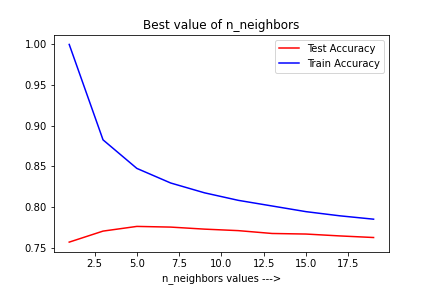
\includegraphics[width=250px]{knn_complexity.png}
    \captionof{figure}{Complexity Curve: \emph{n\_neighbors} value for KNN}
\end{center}
Observing the plot, it shows the same result as the validation accuracy starts to dip after \emph{n\_neighbors}=5.

\subsubsection{Model Evaluation}
Setting \emph{n\_neighbors}=5, we train another KNNClassifier and plot its learning curve as the data increases.
\begin{center}
    \captionsetup{type=figure}
    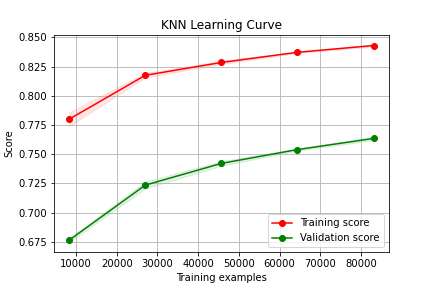
\includegraphics[width=250px]{learning_curve_knn.png}
    \captionof{figure}{Learning Curve for KNN}
\end{center}
Plot shows high variance but decreasing bias with more training data.